\section{Input data description}

 \subsection*{Volume}
 \ttt{EMD-3488}, that can be downloaded from \ttt{PDBE} (\url{http://www.ebi.ac.uk/pdbe/entry/emdb/EMD-3488}). %This volume emulates any other volume that you might obtain experimentally and reconstruct by single particle analyis.
 
 \begin{figure}[H]
  \centering
  \captionsetup{width=.8\linewidth} 
  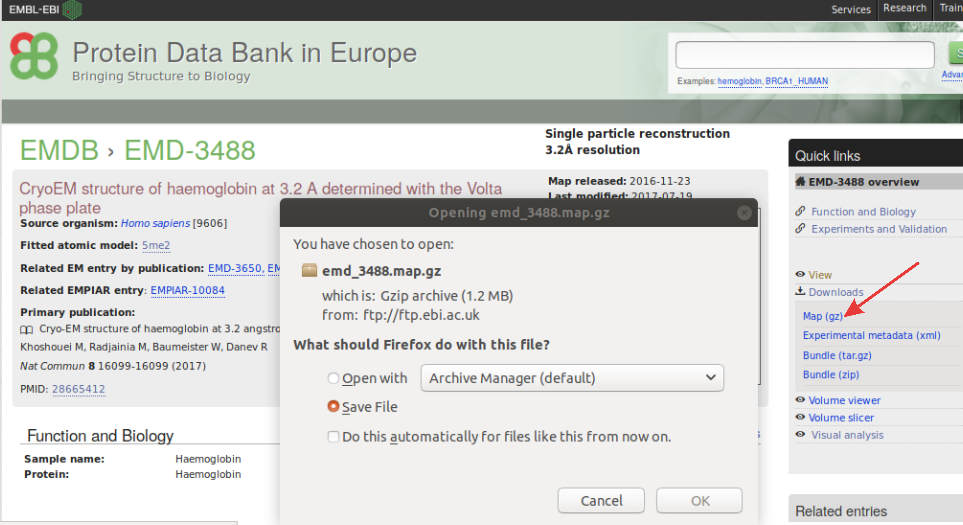
\includegraphics[width=0.95\textwidth]
  {{Images/Fig3}}
  \caption{Downloading the volume from \ttt{PDBE}.}
  \label{fig:PDBE}
  \end{figure}
  
  Once downloaded the volume, unpack it (command line: \ttt{gunzip emd-3488.map.gz}) and save it in your tutorial folder.
 
 \subsection*{Sequences}
 
 The sequences of \ttt{Hgb} $\alpha$ and $\beta$ subunits are included in \ttt{UniProtKB}. Accession numbers are \ttt{P69905} and \ttt{P68871}, respectively. In the following, we show both sequences in fasta format:
 \begin{quote}
   \begin{verbatim}
>sp|P69905|HBA_HUMAN Hemoglobin subunit alpha
MVLSPADKTNVKAAWGKVGAHAGEYGAEALERMFLSFPTTKTYFPHFDLSHGSAQVKGHG
KKVADALTNAVAHVDDMPNALSALSDLHAHKLRVDPVNFKLLSHCLLVTLAAHLPAEFTP
AVHASLDKFLASVSTVLTSKYR

>sp|P68871|HBB_HUMAN Hemoglobin subunit beta
MVHLTPEEKSAVTALWGKVNVDEVGGEALGRLLVVYPWTQRFFESFGDLSTPDAVMGNPK
VKAHGKKVLGAFSDGLAHLDNLKGTFATLSELHCDKLHVDPENFRLLGNVLVCVLAHHFG
KEFTPPVQAAYQKVVAGVANALAHKYH
\end{verbatim}
 \end{quote}

 
 These protein sequences were determined by direct translation from the experimental sequence obtained from complementary \ttt{DNA (cDNA)}, i.e., \ttt{DNA} synthesized or retro-transcribed from messenger \ttt{RNA (mRNA)}. In this way, it is quite unlikely that these sequences included post-translational modifications. Although methionine is added with the translation \ttt{Met-tRNA} initiation factor, the removal of methionine aminoacid from the N-terminus of a polypeptide is a common post-translational modification. Since methionine appears at the N-terminal end of both proteins, we can predict that these are not the polypeptide mature forms and Methionine will be removed in the mature ones that are present in the atomic structures. 
 
 These two sequences can be retrieved from \ttt{UniProtKB} using \scipion\ \scommand{import sequence} protocol, which allows direct download from the database.
 

